\documentclass[dvipsnames,format=sigconf,anonymous=true,review=true]{acmart}

%% \BibTeX command to typeset BibTeX logo in the docs
\AtBeginDocument{%
  \providecommand\BibTeX{{%
    \normalfont B\kern-0.5em{\scshape i\kern-0.25em b}\kern-0.8em\TeX}}}

%% Rights management information.  This information is sent to you
%% when you complete the rights form.  These commands have SAMPLE
%% values in them; it is your responsibility as an author to replace
%% the commands and values with those provided to you when you
%% complete the rights form.
% \setcopyright{acmcopyright}
% \copyrightyear{2018}
% \acmYear{2018}
% \acmDOI{10.1145/1122445.1122456}

%% These commands are for a PROCEEDINGS abstract or paper.
% \acmConference[Woodstock '18]{Woodstock '18: ACM Symposium on Neural
%   Gaze Detection}{June 03--05, 2018}{Woodstock, NY}
% \acmBooktitle{Woodstock '18: ACM Symposium on Neural Gaze Detection,
%   June 03--05, 2018, Woodstock, NY}
% \acmPrice{15.00}
% \acmISBN{978-1-4503-XXXX-X/18/06}


%%
%% Submission ID.
%% Use this when submitting an article to a sponsored event. You'll
%% receive a unique submission ID from the organizers
%% of the event, and this ID should be used as the parameter to this command.
%%\acmSubmissionID{123-A56-BU3}

%%
%% The majority of ACM publications use numbered citations and
%% references.  The command \citestyle{authoryear} switches to the
%% "author year" style.
%%
%% If you are preparing content for an event
%% sponsored by ACM SIGGRAPH, you must use the "author year" style of
%% citations and references.
%% Uncommenting
%% the next command will enable that style.
%%\citestyle{acmauthoryear}


% \usepackage[utf8]{inputenc} % allow utf-8 input
% \usepackage[T1]{fontenc}    % use 8-bit T1 fonts

% \usepackage{amsfonts}       % blackboard math symbols
% \usepackage{amsmath}
% \usepackage{amsthm}
% \theoremstyle{definition}
% \newtheorem{definition}{Definition}

\usepackage{booktabs}       % professional-quality tables
\usepackage{tabularx}
\usepackage{graphicx}
\usepackage{subcaption}
\usepackage{color}
\usepackage{qrcode}


% \PassOptionsToPackage{hyphens}{url} % url is loaded by hyperref
\usepackage{hyperref}
\renewcommand{\sectionautorefname}{Section}
\renewcommand{\subsectionautorefname}{Section}
\renewcommand{\subsubsectionautorefname}{Section}
\newcommand{\definitionautorefname}{Definition}

\usepackage{xspace}
\newcommand{\eg}{e.g.,\xspace}
\newcommand{\ie}{i.e.,\xspace}
\newcommand{\cf}{cf.,\xspace}

% \usepackage{adjustbox}
% \usepackage{wrapfig}
% \usepackage{caption,subcaption}

\newcommand{\achiya}[1]{{\textcolor{red}{[Achiya: #1]}}}
\newcommand{\irina}[1]{{\textcolor{blue}{[Achiya: #1]}}}

\usepackage{listings}
\usepackage{ulem}
%\usepackage{multirow}
%\usepackage{titlesec}

\lstset{
    escapeinside={!}{!},
    language=[x86masm]Assembler,
    basicstyle=\scriptsize,
    keywordstyle=\bfseries,
    commentstyle=\itshape,
    numbers=left,
    numberstyle=\tiny,
    numbersep=6pt, 
    frame=lines,
    breaklines=true
}
\AtBeginDocument{\DeclareCaptionSubType{lstlisting}}
\newcommand{\lstin}[2][]{\lstinline[#1]|#2|}

\usepackage{framed}
\newenvironment{BNF}
  {\captionsetup{type=lstlisting}}
  {}
\usepackage[nounderscore]{syntax}
\setlength{\grammarparsep}{0.1cm}
\setlength{\grammarindent}{2em}

\usepackage[para,flushleft]{threeparttable}

\newcolumntype{L}[1]{>{\raggedright\let\newline\\\arraybackslash\hspace{0pt}}m{#1}}
\newcolumntype{C}[1]{>{\centering\let\newline\\\arraybackslash\hspace{0pt}}m{#1}}
\newcolumntype{R}[1]{>{\raggedleft\let\newline\\\arraybackslash\hspace{0pt}}m{#1}}



\usepackage{multirow}
\usepackage{dblfloatfix}
\usepackage{balance} 


\begin{document}
%% Title
\title{Evolving Assembly Code in an Adversarial Environment}
%Assembly code evolution for CodeGuru players
%%%% Cite as
%%%% Update your official citation here when published 
% \thanks{\textit{\underline{Citation}}: 
% \textbf{Authors. Title. Pages.... DOI:000000/11111.}} 
%}

\author{Irina Maliukov}
\email{irinamal@post.bgu.ac.il}
\orcid{1234-5678-9012}
\author{Gera Weiss}
\email{geraw@bgu.ac.il}
\orcid{0000-0002-5832-8768}
\author{Oded Margalit}
\email{odedm@post.bgu.ac.il}
\orcid{0000-0002-2026-2601}
\affiliation{%
  \institution{Department of Computer Science\\Ben-Gurion University of the Negev}
  \city{Be'er Sheva}
  \country{Israel}
}

\author{Achiya Elyasaf}
\email{achiya@bgu.ac.il}
\orcid{0000-0002-4009-5353}
\affiliation{%
  \institution{Department of Software and Information System Engineering\\Ben-Gurion University of the Negev}
  \city{Be'er Sheva}
  \country{Israel}
}

\renewcommand{\shortauthors}{Maliukov et al.}

\begin{abstract}
In this work, we evolve 8086 assembly code for winning the CodeGuru Xtreme competition. The goal of the competition is to create a survivor---an assembly program that runs the longest in shared memory and is resistant to possible attacks from adversary survivors. Our evolutionary process managed to create a winning survivor against almost each one of the past years' human-written winners. 
For evolving top-notch solvers, we specify a Backus Normal Form (BNF) for the assembly language and synthesize the code from scratch using Grammar-Guided Genetic Programming (G3P). 
We evaluate

Our evolved programs are Previous attempts to evolve low-level programs have focused on evolving single functions with a  Grammatical Evolution (GE), code synthesis, Multi-objective Linear Genetic Programming (MOLGP), Grammar-Guided Genetic Programming (G3P), and PushGP. We chose to use G3P based on typed tree-GP over the others due to the convenience of using Backus Normal Form (BNF) for assembly language in the evolution and being able to perform direct changes on the evolved tree program. Moreover, these approaches weren't fully applied to an unrestricted assembly language.
The domain we focused on is an adversarial environment, where our evolved code faces another code with a goal to over-take it in different possible meanings.
This domain allows us to evaluate the evolved code in an unambiguous way and direct the evolution into achieving accurate goal.
This works shows the evolution of  8086 assembly code in the light of winning CodeGuru competition. CodeGuru Xtreme competition takes place between outstanding high-school students in which the goal is to create an assembly program that runs the longest and is resistant to possible attacks from adversaries. Our evolutionary process managed to create a winning code against almost each one of the past years human-written winners. We believe that using the right fitness evaluation, various goals may be achieved with assembly code evolution as presented in this work.
We evaluate the survivors by running a CodeGuru game against winning human survivors. Our fitness is based on parameters of the individual's earned score, how long it survived, the amount of bytes it wrote, and the rate it wrote them in.
The process was tested against all human-written past winners. The results demonstrate that our evolved programs are able to find weaknesses in the programs that they are trained against and utilize them.  
The reader may ask whether a Large-Language Models (LLMs), like ChatGPT, would be able to achieve similar results. To address this question, we report on an experiment we did, where we provided the game rules and a hand-written individual to ChatGPT and asked it to generate a new survivor to compete it. Even after many attempts and prompt engineering, we could not generate a high-quality survivor that was able to win at any competition. Additional comparison was made to a purely random assembly code generation, which managed to produce viable survivor however, did not manage to produce a winning survivor.
This work has an important application for Cyber-Security. Due to the fact that writing in an assembly language is a necessity in some viruses, by modifying the fitness function, this approach can be used for detecting weaknesses in code and helping fixing them, detecting suspicious adversarial code or on the contrary can be intended to avoid security mechanisms. It also proves the ability to do so without large databases and detailed information. Furthermore, any language that can be represented similarly to assembly using BNF can be used for the evolution. The uniqueness of our work is expressed in the minimal assumptions which are required for the process.
\end{abstract}

%%
%% The code below is generated by the tool at http://dl.acm.org/ccs.cfm.
%% Please copy and paste the code instead of the example below.
%%
% \begin{CCSXML}
% <ccs2012>
%  <concept>
%   <concept_id>10010520.10010553.10010562</concept_id>
%   <concept_desc>Computer systems organization~Embedded systems</concept_desc>
%   <concept_significance>500</concept_significance>
%  </concept>
%  <concept>
%   <concept_id>10010520.10010575.10010755</concept_id>
%   <concept_desc>Computer systems organization~Redundancy</concept_desc>
%   <concept_significance>300</concept_significance>
%  </concept>
%  <concept>
%   <concept_id>10010520.10010553.10010554</concept_id>
%   <concept_desc>Computer systems organization~Robotics</concept_desc>
%   <concept_significance>100</concept_significance>
%  </concept>
%  <concept>
%   <concept_id>10003033.10003083.10003095</concept_id>
%   <concept_desc>Networks~Network reliability</concept_desc>
%   <concept_significance>100</concept_significance>
%  </concept>
% </ccs2012>
% \end{CCSXML}

% \ccsdesc[500]{Computer systems organization~Embedded systems}
% \ccsdesc[300]{Computer systems organization~Redundancy}
% \ccsdesc{Computer systems organization~Robotics}
% \ccsdesc[100]{Networks~Network reliability}

%%
%% Keywords. The author(s) should pick words that accurately describe
%% the work being presented. Separate the keywords with commas.
% \keywords{datasets, neural networks, gaze detection, text tagging}

%% A "teaser" image appears between the author and affiliation
%% information and the body of the document, and typically spans the
%% page.
% \begin{teaserfigure}
%   \includegraphics[width=\textwidth]{sampleteaser}
%   \caption{Seattle Mariners at Spring Training, 2010.}
%   \Description{Enjoying the baseball game from the third-base
%   seats. Ichiro Suzuki preparing to bat.}
%   \label{fig:teaser}
% \end{teaserfigure}

%%
%% This command processes the author and affiliation and title
%% information and builds the first part of the formatted document.
\maketitle

\section{Introduction}
Genetic programming (GP) is a search algorithm inspired by the process of (Darwinian) evolution in Nature. A longstanding challenge in genetic programming is the evolution of computer programs.


In this paper, we present an approach to automatically generate assembly programs using genetic programming. The evolution and evaluation are performed in an adversarial environment in order to evaluate the evolved code in an unambiguous way. The tested adversarial environment is the CodeGuru game (see \autoref{codeguru_explenation}), which is an environment for detecting the longest running assembly program sidelong to adversarial programs which try to win.
Genetic Programming makes a good match for our goal due to its dynamism and integrated ability to improve along the generations. It is a type of evolutionary algorithm that is commonly used to automatically generate computer programs to solve specific problems. GP is inspired by the process of natural selection and evolution in biological systems. Thus, it supplies us the learning curve we need to reach better assembly code than the supplied adversary. The method we used is Grammar-Guided Genetic Programming (G3P), in its typed version. It is an evolutionary computation technique that incorporates Genetic Programming principles, employs a context-free grammar and operates directly with tree-based representations. G3P allows us to evolve assembly programs following grammar type constrains and a defined aim, overtaking adversary in this case. During the evolutionary process with G3P, the evolved code is represented using Abstract Syntax Tree (AST) based on matching assembly Backus normal form (BNF), where the nodes are the BNF's functions and the leafs are the BNF's terminals.
Our grammar representation follows assembly constrains and syntax. The evaluation of the evolved code is done by running a CodeGuru game against top-ranked human-written survivors. The fitness is based on the parameters of individual's earned score, how long it survived, the number of bytes it wrote and the rate it wrote them in. The evolution processes begins with an initial population of 256~randomly generated individuals. A survivor or an individual, is defined as a group of two programs, respectively to the game. Mutations and Cross-overs are performed on the population to reach improvement. Using a tournament method, the best survivors are chosen for the next generation. The evolution terminates when convergence between best and average fitness values of the generations is achieved in addition to monotonic non-increasing winning strike of 200~generations or 3,000~generations are reached, the earlier fulfilled.
We conducted experiments against all human-written past years' winners that showed fine winning results using our Grammar Guided typed-GP method of assembly evolution.
No previous work has been done on the CodeGuru game, except of Bachelor's degree work of~\cite{Darwin8086}. However, some work has been done on assembly code evolution. Previous attempts to evolve low-level programs have focused Grammatical Evolution (GE), code synthesis, Multi-objective Linear Genetic Programming (MOLGP), Grammar-Guided Genetic Programming (G3P) and PushGP. We chose to use G3P based on typed tree-GP over the others due to the convenience of using BNF for assembly language in the evolution and being able to perform direct changes on the evolved tree program. The fact that PushGP is based on type stacks and type matching operators makes it harder to adjust to assembly code and other approaches, as MOLGP, weren't fully applied to unrestricted assembly language.
The successful results of our experiment are applicable to wide aspects, as Cyber-Security, automatic code generation and testing. The fact we used assembly language, which is multi-functional cross-platform low-level language, makes it possible to run on many systems. By changing the fitness calculation following goal-oriented approach, it is possible to evolve assembly code to achieve it.  

\section{Related Work}
\subsection{CodeGuru}
\label{codeguru_explenation}
CodeGuru\cite{codeguru_repo} is a coding competition based on Core War, which is a 1984 programming game created by D. G. Jones and A. K. Dewdney in academic paper (\cite{dewdney1984recreational}).
Short assembly x8086 programs (at most 512 bytes long) of 16-bit commands, called survivors, are loaded into random space on a virtual computer memory arena of size 64KB. Each of the survivors is loaded to a random address, has a individual stack of 2,048 bytes and a full set of registers. The distance between two survivors and an edge of the arena is at least 1,024 bytes.
The goal of each survivor is to defeat all others by staying the last program to run. The last survivor alive is the winner and gets one point. If several survivors stay alive, the point is divided equally between all.
Winning is achieved when opponent's code run illegal commands. One way is to make them run illegal command and another attack is to overwrite the opponent's memory and using it as additional power source to the survivor. A survivor can be disqualified in the following scenarios: 
running illegal command, running a legal assembly command which the engine doesn't support or attempt to access memory address outside of the arena and the survivor's individual stack.
Each battle of the game runs for 200,000 rounds or until only one survivor is left, which ever comes first. In every round, the next command of each survivor is executed in a round-robin fashion. The order of survivor's execution is changed randomly for each game. The game's progress can be monitored by the memory arena image and the score board as seen in the pictures \autoref{fig:CodeGuru}. In most cases, each participant has two programs that collaborate together as a group survivor. There are special techniques in the game implemented by dedicated commands: \texttt{WAIT}x4 increases the speed of a survivor and allows running several opcodes in single round,\texttt{
INT 0x86} implements "heavy bombing" by writing 256 bytes into memory, \texttt{INT 0x87} implements "smart bombing" by re-writing pattern of 4 bytes. All of our experiments, were performed using survivors consisting of two programs.
CodeGuru competition takes place every year from 2005 between outstanding high-school students. Every year the level raises, more sophisticated survivors are written and the harder the competition gets.
\begin{figure}
  \centering
  \begin{subfigure}{0.48\textwidth}
    \includegraphics[width=\linewidth]{images/score_board.jpg}
    \caption{Score board}
    \label{fig:image1}
  \end{subfigure}
  \hfill
  \begin{subfigure}{0.48\textwidth}
    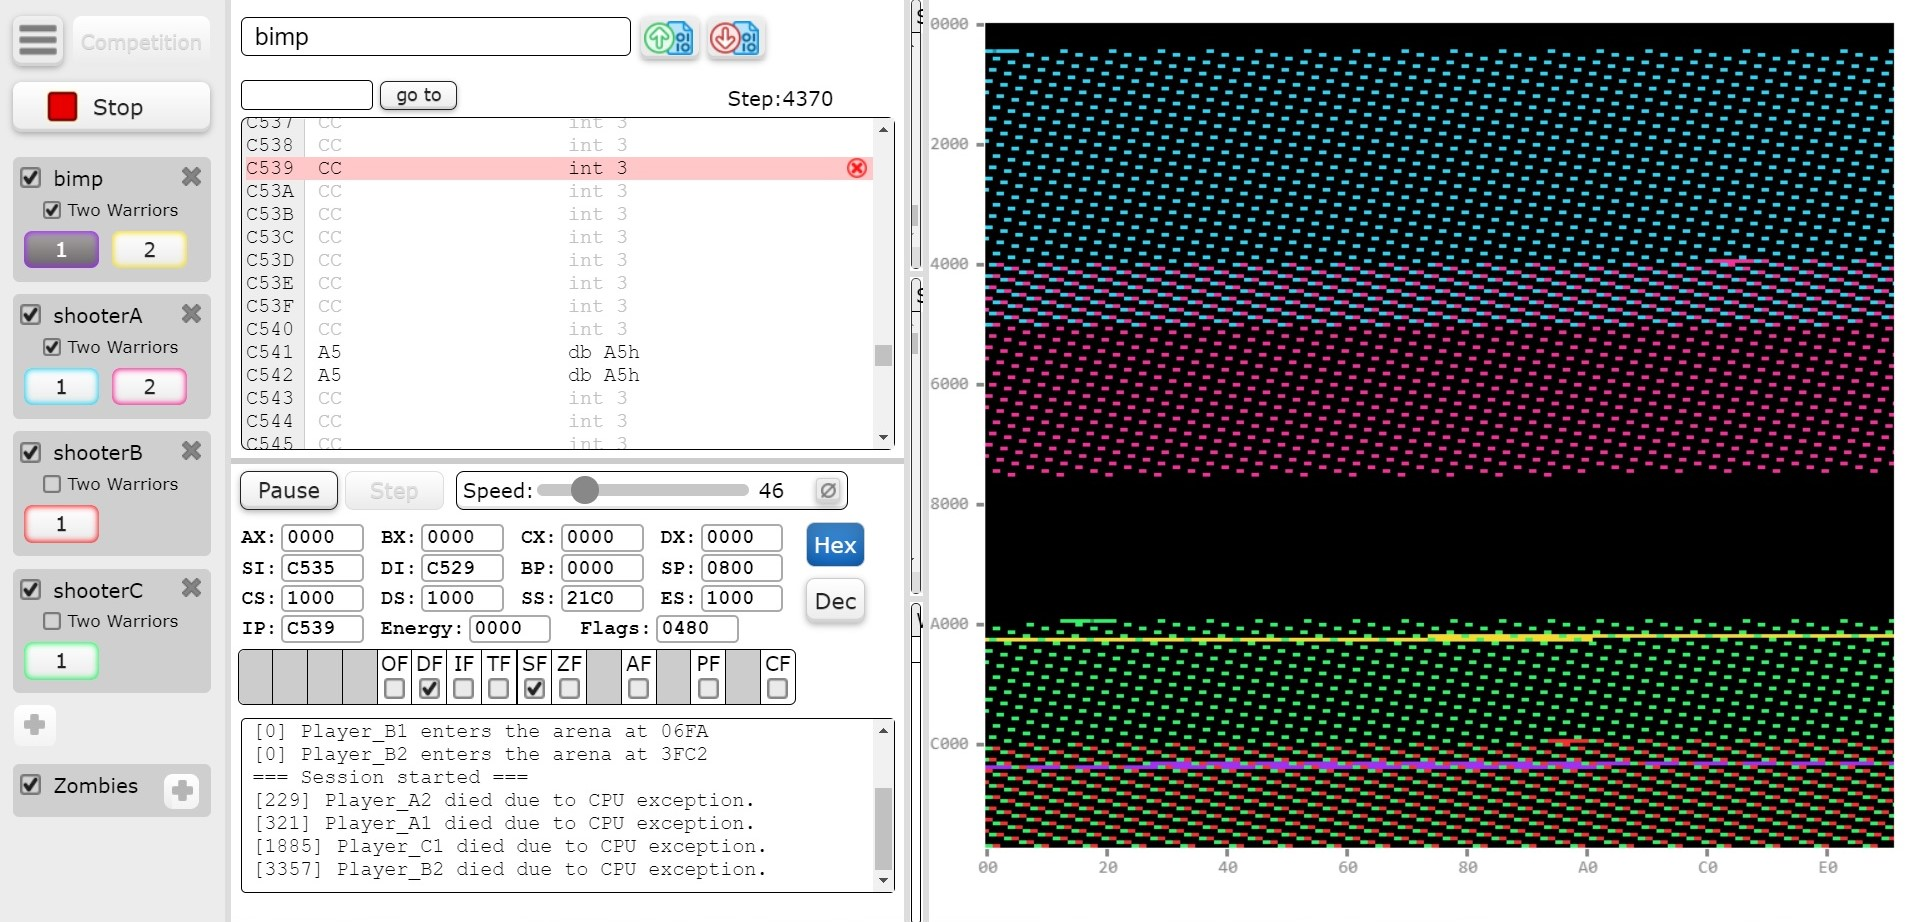
\includegraphics[width=\linewidth]{images/memory_use.jpg}
    \caption{Memory arena}
    \label{fig:image2}
  \end{subfigure}
  \caption{CodeGuru game}
  \label{fig:CodeGuru}
\end{figure}

\subsection{Assembly-like Code Evolution}
\paragraph{Automatic Verilog code generation through grammatical evolution}
This work \cite{ulya2005automatic} suggests some methods for Verilog code generation, which is a hardware description language similar to C programming language. The discussed methods are Genetic programming (provides proper representation mechanism for automatic code generation paradigm due to the representation of the problem as a tree. However, crossover can cause loss of validity), Grammatically based genetic programming (function signatures and return values are defined before the first population and the memory consumption is high) and Probabilistic Incremental Program Evolution (PIPE -- a new node can’t be inserted into the tree without any knowledge about the function and flags of the node). They chose Grammatical evolution (GE) and performed it on specific example of a one bit full adder. Created BNF for the subset of Verilog syntax used in this example, forced assignments to proper expressions and limited nested statements. In spite of the strong bias they employed, the probability of success achieved was only about 5.7\%. 
We expended this idea using a wider BNF representation for a more multiverse language, including enhanced use of mutations and cross overs. Our success rates are higher and our experiments were performed in comparison to human-written code.

\paragraph{Genetic Programming in the Wild: Evolving Unrestricted Bytecode}
This work \cite{Orlov2009Genetic} proposes a method to evolutionary improve existing Java program or software which can be compiled to Java bytecode. They do not use the approach in genetic programming that involves definition of functions and terminals appropriate to the problem. They use evolution of machine code to repair human-written programs. Although Java bytecode acts similar to an assembler, it has simplified representation and does not have direct memory access because it is destined to run on a Java Virtual Machine (JVM). While assembly has very strong correspondence between its instructions and the architecture's machine code instructions and memory. They created a "good" crossover, which ensures a viable bytecode offspring (compiles without error) by holding some conditions on JVM's operand stack, local variables and control flow. Assembly does not have a stack-based architecture like JVM for its execution, so our constrains for viable assembly code will be based on type constrains held during crossover.
In contrast to them, we evolve assembly code from scratch and do not repair or even have access to human-written assembly code to learn from during the evolution.

\paragraph{On the Difficulty of Benchmarking Inductive Program Synthesis Methods} This work \cite{Pantridge2017On} compares Flash Fill (Microsoft Excel feature which uses version-space algebras to perform program synthesis from examples on string manipulation tasks), MagicHaskeller (synthesizes functional Haskell programs
through an exhaustive search of programs with the correct type signatures. Uses Monte-Carlo algorithm to remove semantically equivalent programs from the search space), TerpreT (probabilistic programming language that is designed for inductive program synthesis), and two forms of genetic programming -- PushGP (evolves programs in a Turing complete, stack based language called Push\autoref{PushGP}) and Grammar Guided Genetic Programming (G3P system’s grammar is composed of a separate context-free grammar for each data type, grammar for the structure of the program and skeleton of signature specifies the inputs to the function and the return statement (see subsection~\autoref{GrammarGP})). The comparison focused on the possibility of producing a program that passes all tests, for all training and unseen testing inputs. It was made on problems some of usually approached using machine code or assembly language (Basic Execution Models Problems), while others usually approached using highlevel languages (General Program Synthesis Benchmark Suite). In low-level field, the system that performed the best was TerpreT, while sadly there were no gathered results for G3P. In high-level field, both genetic programming systems outperformed the others.
We want to follow Grammar Guided Genetic Programming in the untested field of low-level languages with the needed modification to match it to assembly language GP.

\paragraph{Automatic Code Generation for MicrocontrollerBased System Using Multi-objective Linear Genetic
Programming}
This work \cite{Serruto2017Automatic} proposes the application of
multi-objective linear genetic programming for automatic
generation of some specific assembly driver routines. For fitness evaluation, they maximize a function to each bit of the binary result or the timing diagram of each used micro-controller Port pins, respectively to the targeted routine. The used architecture was 8051 micro-controller assembly, which is similar to x8086 we use. The evolved micro-controller programs did not contain jump instructions because they could form infinite loops, in contrast to our wish to include them in the generated code. They adopted LGP chromosome representation with dynamic size because in evolutionary process instructions of micro-controller program are in machine language, which is an imperative language. They tested their results using two multi-objective optimization algorithms: EMOEA and NSGAII and compared them to written-by-human programs taken from micro-controller assembly language programming courses. The results showed that the automatic generated micro-controller code, for specific tasks, can compete with a human programmer with smaller code size or faster execution. 
In our work, we aim to create more general assembly code, including jumps and loops. The presented results strengthens the possibility of achieving our goal. 

\paragraph{Genetic Programming-Based Code Generation for
Arduino}
This work \cite{Ferrel2020Genetic} similarly to the previous one, presents methodology for writing programs for Arduino board using an automatic generator of assembly language routines based on cooperative co-evolutionary multi-objective linear genetic programming algorithm. They decompose the problem into sub-components, generate about 73\% of the program and the remaining 27\% which are the main program and some initial configuration routines are manually written. The automatic generation also requires an input-output table for the routine. The multi-objective genetic programming algorithm aims that the generated table is equal to the required one. Thus, in this work, multi-objective optimization seeks to maximize the
vector of objective functions. Each one corresponds to a pin of a Port or one bit of the objective code, depending on the generated routine purpose. One of the pointed limitations of the proposed methodology is that the application of it depends on the existence of
sub-tasks that are described by input-output tables.
In our case, we cannot break the goal of winning a opponent to sub-tasks without reading its code first, which we avoid. In addition, there isn't a clear way to represent a wining result in our case using input-output table. We need to completely automatically evolve a winning program, which makes the used method incompatible in our case.

\paragraph{Stepping Stones to Inductive Synthesis of Low-Level Looping Programs}
This work \cite{Rosin2019Stepping} presents synthesis of low-level programming languages, close to assembly language, looping programs from input/output examples. They targeted simplified low-level language where each instruction consists of an opcode and a single operand. Their method is Delayed Acceptance hill-climbing. Rather than immediately accepting an update to the current-best candidate solution, continue to gather additional candidates for a period of I steps, and then accept the best found during that period. This is done in order to avoid local optimums. They compared their results with TIS-100, which is an assembly language programming game for players who tracked the best programs they could find for each puzzle. One of the categories is to minimize the number of instructions and their code matched the best reported program.
Their results show that it is possible for synthesizing assembly-like programs to compete with human-written ones. We want to expend this approach by evolving assembly code from scratch, worthy to over take human-written code.

\paragraph{Recent Developments in Program Synthesis with Evolutionary Algorithms}
This work~\cite{domonik2021recent} discusses recent research directions in GP filed. Between the discussed themes, the most relevant for our goal were the following: Stack based GP - usually PushGP (see subsection~\autoref{PushGP}), Grammar guided GP (see subsection~\autoref{GrammarGP}) and Linear GP (uses registers for calculations and direct memory access).
This works presents useful ideas of various research directions to achieve our goal of assembly code evolution. Each of them is discussed in this paper and explained why or why no is it suitable for us.

\subsection{Grammar-Guided Genetic Programming (GGGP | G3P)}
\label{GrammarGP}
\paragraph{Grammatical Evolution (GE)}
Grammatical Evolution (GE) may be considered as an instance of Grammar-Guided Genetic Programming (G3P). In GE, an evolutionary algorithm utilizes a grammar, often in BNF form, to precisely define the syntax of candidate solutions. It combines principles from Genetic Programming while utilizing a fixed-length binary string representation. This binary string is then mapped to a syntax-compliant solution, thanks to a specific decoding mechanism as described here \cite{ONeil2004piGE}. One of the key advantages of GE is its ability to evolve programs in any language defined using a context-free grammar. On the other hand, Grammar-Guided Genetic Programming is also an evolutionary computation technique that incorporates Genetic Programming principles and employs a context-free grammar. Unlike GE, which uses a linear genome representation, G3P primarily operates directly with tree-based representations. This characteristic offers several advantages, as it allows for convenient direct manipulation and generation of tree structures. Consequently, applying genetic operators like crossover and mutations, as well as enforcing type constraints, becomes simpler and more intuitive in G3P. In our case, where assembly language can be conveniently represented using BNF and tree form, G3P emerges as the more suitable approach. The inherent direct modifications on the tree structures align well with the requirements to evolve assembly code. This makes G3P an advantageous choice for our needs.

\paragraph{A Grammar Design Pattern for Arbitrary Program Synthesis Problems in Genetic Programming} This work \cite{Forstenlechner2017Grammar} proposed the concept to approach program synthesis using a standard tree-based grammar guided GP system (G3P), with a few additions of Grammar and Skeleton to make it flexible to evolve, while focusing on Python. The skeleton here is the part of the design pattern that is executed in the end to evaluate the individual.
In our work, we will use skeletons in a different way. They will be used as the functions in our BNF and programs will be generated according to their structure. The printing of the assembly program will be guided by this skeleton tree. In contrast to the suggested approach in this work, our assembly grammar representation isn't tailored to our specific domain. It is flexible and consists of various assembly opcodes and operands and patterns which can be applied to any program.

\paragraph{}
The following website \cite{Haas2022GGGP} contains prototype code examples and the results they produced on some problems (like, OpenAI Gym: Cartpole-v1) using two grammar-guided genetic programming methods CFG-GP (context-free grammar GP) and GE. This site aims to improve CFG-GP and GE and additionally implement three more recent approaches that supposedly have better performance: piGE, DSGE and WHGE. In addition, it aims to apply the best grammar-guided genetic programming method in a real-world setting.
Currently, they create a tailored grammar representation and a solution skeleton for the problem they want to solve and run evolutionary algorithm until the desired solution is evolved. This is done using alogos python package, written by the same author. We haven't found explanation to the genetic operators they use in the process.
In our case, we do not want to limit our generated assembly code to a specific output program, thus our supplied grammar is much more general and subject to change than the presented here. Moreover, our skeletons contain only assembly general patterns such as a loop and not specified function structure like seen in this github page.

\paragraph{piGE}
\label{piGE}
$\pi$Grammatical Evolution as described in \cite{ONeil2004piGE}, is a position independent version of GE, where the genome is used to specify which nonterminal will be developed next, in addition to specifying the rule that will be applied to it. This enables to manipulate the order of derivation steps and not only apply them, as usual, from left to right. The idea is to break the dependency chain into smaller fragments that can be exchanged between appropriate contexts, similarly to sub-trees in GP. To preserve type constrains, there is an approach in $\pi$GE to only allow choices between non-terminals of the same type and simply change their position in the developing program. $\pi$GE showed better performance than GE over standard GP problems.
As we use GP, the sub-trees satisfy the main goal of this work, which was to facilitate the creation of smaller, functional, building blocks in order to ease their preservation and enhance the scalability of GE to harder problem domains. Sub-trees can be created and inserted to our individuals using our mutation implementation or switched between individuals in our crossover implementation, while preserving the root type.

\paragraph{DSGE}
\label{DSGE}
Dynamic Structured Grammatical Evolution as presented in \cite{Lorenco2018Structured} is a techniques which aims to cancel SGE's need to pre-process input grammar according to supplied maximum levels of recursion in order to remove it from the grammar. SGE handles one of GE's main drawbacks, the redundancy (the tendency of not using portions of the genotype for mapping
into the phenotype) and locality (the tendency of mapping genotypic neighbors to
phenotypic neighbors) of the representation. DSGE outperforms earlier SGE by canceling the need to pre-process input grammar. This is done by representing the individuals using a variable length representation, where just the number of needed derivations are encoded. This is instead of computing and generating the maximum number of derivations for each of the grammar’s non-terminal symbols and eliminates the need to create intermediate symbols to deal with recursive rules. To limit the genotype size, a maximum tree-depth needs to be defined.
As we chose to use G3P instead of GE, we avoid the problem of redundancy and locality of the representation. In addition, we do not pre-process the grammar and the tree depth limitation is rooted in tree-GP, which we use.

\paragraph{WHGE}
Weighted Hierarchical Grammatical Evolution as presented in \cite{Bartoli2018Weighted}, is an approach for mapping genotypes to phenotypes. In GE, genotypes are bit strings while phenotypes are strings of a language
defined by a user-provided context-free grammar. They mapping uses hierarchical relations between nodes of a derivation tree to impose the desired structure on the genotype and encodes grammar symbols with a varying number of bits, based on their relative expressive power. The technique was tested on a set of selected benchmarks, comparing the results to $\pi$GE\autoref{piGE} and SGE\autoref{DSGE} and outperformed them in some of the discussed aspects.
This seems to be relevant only to GE, thus the impact on our approach is minimal.

\subsection{PushGP}
\label{PushGP}
PushGP as presented in \cite{Spector2002Genetic} is a genetic programming system, which evolves programs expressed in the Push programming language. In Push, when a literal (such as the integer) is executed, it is pushed onto the stack of the appropriate data type (in this case, the integer stack). When an instruction is executed, all of the arguments that it requires are popped out of the appropriate stacks and the results are pushed onto the appropriate stacks. Push’s syntactic minimality stems from the fact that arguments are passed between instructions via typed stacks, rather than through the relative positions of instructions and arguments in
a program’s text which ensures type compatibility. Push implementations have been developed in at least the following languages: C++, Clojure, Common Lisp, Elixir, Forth, Java, Javascript, Racket, Ruby, Scala, Scheme, swift and Python \cite{Pantridge2017PyshGP}. 
None of them is a low-level programming language like assembly.

\paragraph{Functional Code Building Genetic Programming}
This work \cite{edward2022functional} presents LISP program evolution using CBGP (code building genetic programming). CBGP is an new approach to recent years program synthesis methods, like PushGP and Grammar Guided Genetic Programming and is inspired by them both. It is a method of evolving human-readable programs using a stack-based compiler. CBGP uses a variable length linear genome, which is translated into a type-safe AST using a compilation process. Specifically, the plushy genome structure. The categories of genes that can be in a genome sequence are literals, variables, local variables, stack instructions and structure tokens. 
The types in CBGP are based on Hindley-Milner type system, which allows to infer the most general type of a given program. 

In order to apply PshGP or CBGP to assembly language, it is necessary to change the native type approach. In assembly, there is no concept of return value type nor a type matching operators or operand. The only native type applicable components might be constant values. Perhaps, they can be summarized to byte, word or double-word with no importance to the original type of bit sequence they hold inside. Operators can be divided according to the number of operand they receive and their size. Operands can be typed by the purpose of the register and its size. Return value concept should be modified according to the operand where the command's output is saved in. There is no implementation of PushGP in an assembly like language and there is no easy way to express assembly using Push programming language. This will require significant modifications and re-implementations of existing PushGP variations due to the change of type perception. Thus, we chose a different approach of tree-GP, which many PushGP systems have used techniques borrowed from it, including tournament selection and crossover based on the swapping of
sub-expressions.


\section{Method}
In this work, we utilize genetic programming to evolve assembly programs in adversarial environment. Our domain is an adversarial environment of a CodeGuru game for two (or more) players, where one is the evolved program and the other is human-written. The goal is for the evolved code to win its adversary.
Genetic Programming or GP, is a type of evolutionary algorithm that is used to automatically generate computer programs to solve specific problems. It is inspired by the process of natural selection and evolution in biological systems. GP can be divided into typed and non-typed methods. In the first one, each node in the program has explicitly defined type and the evolution process ensures type consistency. The second one, does not enforce any type constraints on the programs being evolved. Our chosen method was Grammar-Guided Genetic Programming (G3P), in its typed version. It is an evolutionary computation technique that incorporates Genetic Programming principles, employs a context-free grammar often in BNF form and operates directly with tree-based representations. G3P allows us to evolve assembly programs following grammar type constrains and a defined aim, overtaking adversary in this case. During the evolutionary process with G3P, the evolved code is represented using Abstract Syntax Tree (AST) based on matching assembly BNF representation. Utilizing genetic programming techniques and operators, resulted in a winning evolved program. The following paragraph describes the used grammar, fitness and provides overview on the evolutionary process.

To evolve assembly programs, we developed a Backus normal form (BNF) representation for the assembly language. BNF is a meta-syntax notation for context-free grammars, consisting of derivation rules. Since assembly is a symbolic programming language, it can be represent using it. The terminals are opcodes and operands, as described in \autoref{table:1_terniaml_set} and the functions are structures in the language, as described in \autoref{table2_function_set}. We defined our types and derivation rules based on assembly language constrains. For example, a command consisting of an opcode which takes only one operand. This definition combines naturally with typed tree-GP and the code evolution. Its important to note the assembly grammar presented here is general and can match any assembly x8086 code, apart from the op\_special terminals, which are specific to CodeGuru. There are assembly commands which the game's engine doesn't support and were left out of the grammar to preserve legal programs.

The evaluation of the survivors was done by running a CodeGuru game of 200 battles against human-written winning survivor from past years competitions. The game's engine is an open java source code which we modified in order to produce more information about the survivors, in addition to the final scores it provides originally. It can be found here \cite{ModifiedEngine}. All the following described parameters are used in the fitness calculation:
score: the average score the survivor earned in all played games. The score encourages the evolution of survivors which earn higher scores.
$score = \frac{\sum_{i=1}^{games} score_i}{games}$ 
lifetime: normalized number of average rounds the survivor managed to stay alive in all played games. This parameter encourages the evolution of legal programs which keep running without performing illegal action.
$lifetime = \log_{10} max(1, \frac{\sum_{i=1}^{games} reached\_round_i}{games})$
written bytes: normalized number of average new bytes\footnote{The write was performed on a memory fragment which the last one to write in wasn't the survivor itself} the survivor wrote to memory in all played games\\
$written\_bytes = \log_{10} max(1, \frac{\sum_{i=1}^{games} written\_bytes_i}{games})$
writing rate: the average rate the survivor wrote new bytes in all played games
$writting\_rate = \frac{\sum_{i=1}^{games} written\_bytes_i}{max(1, \sum_{i=1}^{games} reached\_round_i)} * \frac{1}{games}$. The number of written bytes and the rate of their write encourage evolution of programs that write on different places in memory, which enhances the chance of damaging opponents.
Each of the above elements has different impact on the desired outcome of a winning survivor. We refer to the score parameter as the most significant one due to the fact it reflects the performance of our evolved individual compared to the adversary it is evaluated against. The fitness formula which performed the best was: $\mbox{Fitness} := 2 * \mbox{score} + 0.02 * \mbox{lifetime} + 0.03 * \mbox{written\_bytes} + 0.01 * \mbox{writing\_rate}$. It produces fitness value in the range of [0, 2.5] which is comfortable to use and doesn't produce sharp deviations.

Our evolution process generates initial population of 256 random individuals using Grow method. Grow method produces trees of different sizes, while not reaching the maximum depth, a node is chosen from functions and terminals and in the maximum depth, the choice is made only from the terminals. In our case, the maximum depth was defined as 22. We refer to an individual as a group of two survivors, respectively to CodeGuru game. Each one is represented by an abstract syntax tree (AST), which is a tree representation of the abstract syntactic structure of the code. The tree nodes are the BNF’s functions and the leafs are the BNF’s terminals. 
Operators, such as crossover and mutations, were applied on the survivors during the evolution process.
The crossover is performed by randomly choosing a node and replacing its sub-tree with sub-tree of a root of the same type, taken from another tree.
The mutation is performed similarly to the crossover, only the replacement is done with a randomly generated sub-tree with a root of the same type.
Additional operators duplicate the best tree between both of the same individual (duplication mutation) or switch trees between two individuals (replacing mutation).
Statistical analysis was performed on several evolutionary runs in order to evaluate the operators. Each of them was applied on the best individual and on one random individual every 5 generations for 100 repeats. All of the operators had weak improvement effect on the best individual, as expected. However, the results on the random one showed an average improvement chance of about 50\% during the process.
The data of improvement probability created a noticeable sine wave as seen in~\autoref{fig:Improvement_chance}.
\footnote{I don't see it -- it looks like randome with correlation downwards.}
\begin{figure}
  \centering
  \begin{subfigure}{0.48\textwidth}
    \includegraphics[width=\linewidth]{images/crossover_improvment.png}
    \caption{Crossover improvement probability}
    \label{fig:cross}
  \end{subfigure}
  \hfill
  \begin{subfigure}{0.48\textwidth}
    \includegraphics[width=\linewidth]{images/muatation_improvement.png}
    \caption{Mutation improvement probability}
    \label{fig:mut}
  \end{subfigure}
  \begin{subfigure}{0.48\textwidth}
    \includegraphics[width=\linewidth]{images/duplication_improvment.png}
    \caption{Duplication improvement probability}
    \label{fig:dup}
  \end{subfigure}
  \hfill
  \begin{subfigure}{0.48\textwidth}
    \includegraphics[width=\linewidth]{images/replacing_improvement.png}
    \caption{Replacing improvement probability}
    \label{fig:rep}
  \end{subfigure}
  \caption{Operators improvement probability}
  \label{fig:Improvement_chance}
\end{figure}

Mutation was performed in the probability of 0.7, crossover in the probability of 0.3, duplication and replacing mutations are performed in 0.2 probability each. These percents yielded the best outcome, corresponding to the thumb-rule in GP where mutation probability should be higher than crossover's.
Using a tournament method with size of 4, the best survivors were chosen for the next generation. We did not use elitism in our process. Elitism refers to the ability of forwarding several best individuals of a generation to the next one, as they are, without applying operators on them. We decided to avoid it in order to keep the population diverse and avoid forwarding survivors which accidentally won and are not truly good.
The evolution was set to terminate when convergence between best and average fitness values is achieved in addition to monotonic non-increasing winning strike of 200 generations or 2,000 generations are reached, the earlier fulfilled condition.
Our code is based on EC-KitY library presented in \cite{eckity2022git} and the entire assembly evolution code can be found in \cite{AssemblyCodeGeneration}. The code is written in python and can run in multiprocessing or multithreading configuration of the executor's choice. The engine and the adversary survivor need to be placed in the corresponding directories.
We conducted our experiments against all human-written survivors which won in past years' competitions. The evolved survivors manage to find a weakness in their adversaries code, without having access to it, and utilize the finding to win the battle. In all of the cases, fine winning results were achieved using our Grammar Guided typed-GP method of assembly evolution.

%\clearpage
\begin{table*}
\centering
\begin{tabular}{|c|p{11.6cm}|} 
\hline
\multicolumn{1}{|c|}{\textbf{BNF type}} &
\multicolumn{1}{c|}{\textbf{Terminals}} \\ [0.5ex] \hline\hline
$<reg>$ & ax, bx, cx, dx, si, di, bp, sp \\ \hline
$<half\_reg>$ & ah, al, bh, bl, ch, cl, dh, dl \\ \hline
$<addres>$ & [bx], [si], [di], [bp] \\ \hline
$<pop\_reg>$ & ax, bx, cx, dx, si, di, bp, WORD [bx], WORD [si],  WORD [di],  WORD [bp], ds, es \\ \hline
$<push\_reg>$ &  ax, bx, cx, dx, si, di, bp, WORD [bx], WORD [si],  WORD [di],  WORD [bp], ds, es, cs, ss \\ \hline
$<const>$ & [(2*i) for i in range(-10, 133)], @start, @end, 65535, 0xcccc \\ \hline
$<op>$ & nop, stosw, lodsw, movsw, cmpsw, scasw, pushf, popf, lahf, stosb, lodsb, movsb, cmpsb, scasb, xlat, xlatb, cwd, cbw, cmc, clc, stc, cli, sti, cld, std\\ \hline
$<op\_single>$ & div, mul, inc, dec, not, neg \\ \hline
$<op\_double>$ & cmp, mov, add, sub, and, or, xor, adc, sbb, test \\
\hline
$<op\_jmp>$ & jmp, jcxz, je, jne, jp, jnp, jo, jno, jc, jnc, ja, jna, js, jns, jl, jnl, jle, jnle, loopnz, loopne, loopz, loope, loop \\ \hline
$<op\_rep>$ & rep, repe, repz, repne, repnz \\ \hline
$<op\_function>$ & call, call near, call far \\ \hline
$<op\_special>$ & wait wait wait wait, wait wait, int 0x86, int 0x87  \\ \hline
$<op\_pointer>$ & lea, les, lds\\ \hline
$<op\_ret>$ & ret, retn, retf, iret\\ \hline
$<op\_push>$ & push\\ \hline
$<op\_pop>$ & pop\\ \hline
$<op\_double\_no\_const>$ & xchg\\ \hline
$<op\_shift>$ & sal, sar, shl, shr, rol, ror, rcl, rcr\\ \hline
$<section>$ & "" \\ \hline

\end{tabular}
\caption{Terminals definitions}
\label{table:1_terniaml_set}
\end{table*}

\begin{table}[!ht]
\centering
\begin{tabular}{p{15.6cm}} 
<section> ::= <label> <section> <backwards\_jump> <section>
\\ 
<section> ::= <label> <section> <backwards\_jump>
\\ 
<section> ::= <section> <forward\_jmp><section> <label> <section>
\\ 
<section> ::= <label> <section> <call\_func> <backwards\_jump> <label> <section> <return>
\\ 
<section> ::= <op\_double> <reg>  <reg | const | address> <section>
\\ 
<section> ::= <op\_double> <address> <reg | half\_reg> <section>
\\ 
<section> ::= <op\_double> <half\_reg> <half\_reg | const | address> <section>
\\ 
<section> ::= <op\_double> <WORD | BYTE> <address> <const> <section>
\\ 
<section> ::= <op\_pointer> <reg> <address> <section>
\\ 
<section> ::= <op\_double\_no\_const> <reg> <reg | address> <section>
\\ 
<section> ::= <op\_double\_no\_const> <half\_reg> <half\_reg | address> <section>
\\
<section> ::= <op\_single> <reg | half\_reg> <section>
\\ 
<section> ::= <op\_single> <WORD | BYTE> <address> <section>
\\ 
<section> ::= <op\_function> <address> <section>
\\ 
<section> ::= <op | op\_special> <section>
\\ 
<section> ::= <op\_rep> <op> <section>
\\ 
<section> ::= <op\_push> <push\_reg> <section>
\\ 
<section> ::= <op\_pop> <pop\_reg> <section>
\\ 
<section> ::= jmp <reg | address> <section>
\\ 
<section> ::= dw 0x<const> <section>
\\ 
<section> ::= <op\_shift> <reg | half\_reg> <cl | 1> <section>
\\
<call\_func> ::= call l<const> <section>
\\
<return> ::= <op\_ret> <section>
\\ 
<label> ::= l<const> <section>
\\ 
<forward\_jump> ::= <op\_jmp> l<const> <section>
\\ 
<backwards\_jump> ::= <op\_jmp> l<const>-1 <section>
\\
<address> ::= [<address> + <const>] 
\\ 

\end{tabular}
\caption{Functions definitions}
\label{table2_function_set}
\end{table}

\section{Results}
We evaluated our evolved programs using the fitness calculation described previously. During the training, each evaluation included CodeGuru game of 200 battles, when a wining result was considered as a score higher than 0.5. The test step was conducted the same way for the best resulted individual and the validation was performed on the same individual using the web CodeGuru engine, which runs 1,000 battles and a win is considered as a a win in more than 500 battles. We evaluated our performance against all previous years last phase winners which can be found here \cite{codeguru_repo}, the results are brought in  \autoref{table:test_results}.

\begin{table}[!ht]
\centering
\begin{tabular}{|c|c|c|} 
\hline
\multicolumn{1}{|c|}{\textbf{Human-written adversary}} &
\multicolumn{1}{c|}{\textbf{Test score}} &
\multicolumn{1}{c|}{\textbf{Web score}} \\ [0.5ex] \hline\hline
Zeus 2006 & 0.73 & 675 \\ \hline
HutsHuts 2007 & 0.9933333 & 974.67\\ \hline
APOCALYPSE 2008 & 0.79 & 762\\ \hline
XLII 2009 & 1.0 & 999.5\\ \hline
FSM 2010 & 0.475 & 348.5\\ \hline
Mamaliga 2011 & 0.73 & 676.5\\ \hline
Zorg 2012 & 0.77 & 737.17\\ \hline
Snake 2013 & 0.925 & 895\\ \hline
IamAramAcham 2014 & 0.909836 & 674 \\ \hline
Paranoia 2014 & 1.0 & 997\\ \hline
SilentError	2015 & 0.845 & 734\\ \hline
LoudBugFix 2016 & 0.525 & 503.83 \\ \hline
Memz 2017 & 0.98083335 & 980.5\\ \hline
Barvaz'sAngles 2018 & 0.995 & 995.67\\ \hline
Nuki'sDemons 2019 &  0.995 & 991.5 \\ \hline
GreeniEs 2020 & 0.99 & 984 \\ \hline
BlocksOfGuru 2021 & 0.8125 & 736.67\\ \hline
TheHeapMen 2022 & 0.675 & 497.5\footnote{most cases websocre is 1000 times test score, but not here, why?)} \\ \hline
\end{tabular}
\caption{Test and web game results}
\label{table:test_results}
\end{table}

As reflected in~\autoref{table:test_results}, our evolution process managed to evolve assembly program which won nearly all past years human-written winners, with 94.4\% wining chance. Moreover, each one who won in the test phase, respectively won in the validation. This was achieved by using general assembly patterns and using adversarial environment for evaluation, while the adversary's code was never accessible to ours.
The inspection of the evolved winners, raised an interesting fact that the evolved survivors manage to win complex and long survivors using a relatively small code fragment. Although GP frequently evolves long code, sometimes only a small part of it is achieved in the program run flow and yet manages to win. This reinforces the fact the evolution process was able to find Achilles' heel, a weakness, of the opponents code and utilize it for its benefit. Let us elaborate about additional discovered features.

\subsection{Utilizing Achilles' heel}
One of the clearest examples is of Zorg 2012 winner, a part of brought in \autoref{oroginal_zorg}. It writes an important code fragment for its future run on memory address zero in line 23 of its first part. The evolution process notices it and overrides this memory cell using addressing di which holds the value zero, depriving Zorg from wining. As seen in the evolved winner's line 14 of first and second code \autoref{evolved_zorg}. The first generation of this evolution started with nearly zero score and in about 100 generations the average score of the population was a winning score. It happened due to the application of the operators which enabled the discovery of the weakness. As mentioned, Zorg's code is significantly longer and more complicated than the evolved fragment which managed to overtake it. The evolved survivor manages to win Zorg in 77\% of the cases despite the weakness finding due to the randomness in the game's execution order.

\lstnewenvironment{assembly}{%
  \lstset{
    escapeinside={!}{!},
    language=[x86masm]Assembler,
    basicstyle=\small,
    keywordstyle=\bfseries,
    commentstyle=\itshape,
    numbers=left,
    numberstyle=\tiny,
    numbersep=0pt, 
    frame=lines,
    breaklines=true
  }%
}{}

\begin{figure}
\centering
\begin{subfigure}{0.48\textwidth}
    \begin{assembly}
    JMP 0xC1
    ADD WORD SI, 0xB4
    MOV CX, 0x6
    MOVSB
    REP MOVSW
    ADD WORD SI, 0x60
    MOV CX, 0xB
    REP MOVSW
    MOV BP, 0xFF
    !\sout{db 0xE9, 0xE7, 0x00}! JMP 0xEA
    MOVSW
    MOVSW
    MOVSW
    ADD WORD DX, 0x17A8
    MOVSW
    DEC BP
    MOVSW
    MOVSW
    !\sout{db 0x74, 0x0F}! JZ SHORT 0x11
    MOV SI, AX
    NOP
    ADD AX, 0x95
    !\textcolor{red}{\textbf{MOV BYTE} [0x0], 0xBE}!
    MOV [0x1], SI
    MOV WORD [0x3], 0xC289
    MOV BYTE [0x5], 0xE9
    MOV [0x6], AX
    ...
    \end{assembly}
    \caption{Zorg part 1}
\end{subfigure}
\hfill
\begin{subfigure}{0.49\textwidth}
    \begin{assembly}
    JMP SHORT 0x6C
    MOV SI, AX
    PUSH ES
    PUSH CS
    POP ES
    MOV BX, 0xDB31
    MOV CX, 0xE3FF
    MOV AX, 0x789
    MOV DX, 0xFEEB
    INT 0x87
    POP ES
    MOV DX, SI
    MOV BP, 0x17A8
    MOV CX, 0x3F3
    MOV AX, 0xAB53
    MOV BX, 0xCCA5
    PUSH CS
    PUSH ES
    PUSH DS
    POP ES
    POP DS
    POP SS
    MOV SP, DX
    ADD WORD SP, 0xF3
    MOV DI, DX
    XOR SI, SI
    STOSW 
    ...
    \end{assembly}
    \caption{Zorg part 2}
\end{subfigure}
\caption{Zorg 2012 winner}
\label{oroginal_zorg}
\end{figure}

\begin{figure}
\centering
\begin{subfigure}[t]{0.48\textwidth}
    \begin{assembly}
    @start:
    and cl, [bx + 0x68 + 0x104 + 0x246]
    div WORD [bx]
    l8293849:
    rcl dl, cl
    rcl ax, 1
    rol si, cl
    push WORD [si]
    shl dh, cl
    l8293850:
    and WORD [di + 0x222], 0x92
    wait
    wait
    !\textcolor{red}{\textbf{mov WORD} [di], 0x196}!
    jns l8293850
    @end:
    \end{assembly}
    \caption{Evolved survivor part 1}
\end{subfigure}
\hfill
\begin{subfigure}[t]{0.49\textwidth}
    \begin{assembly}
    @start:
    sub bh, [bx + 0x30 + @start]
    div WORD [bx]
    l8293858:
    rol dl, cl
    shr di, 1
    dw 0x144
    push ds
    sbb dl, 0x34
    sar ax, cl
    l8293859:
    and WORD [si + 0x246 + 0x230], 0x264
    push bx!\footnote{was the push/pop a pattern?}!
    !\textcolor{red}{\textbf{pop WORD} [di]}!
    and WORD [si + 0x206 + 0x202 + 0x220 + 0x-14 + 0x-20 + 0x32], 0x144
    jmp l8293859
    @end:
    \end{assembly}
    \caption{Evolved survivor part 2}
\end{subfigure}
\caption{Evolved survivor against Zorg}
\label{evolved_zorg}
\end{figure}

\subsection{Concentrated vs. Scattered memory writes}
The experiments express the strength of evolutionary algorithms in discovering improvement using the operators. All the histograms in \autoref{fig:Histograms} reflect sharp jumps in the best fitness value graph, indicating of good gene findings. This moves the population forward for evolving winning individuals. 

\begin{figure}
  \centering
  \begin{subfigure}{0.33\textwidth}
    \includegraphics[width=\linewidth]{images/blocksofguru_hist.png}
    \caption{BlocksOfGuru 2021}
    \label{fig:hist1}
  \end{subfigure}
  \hfill
  \begin{subfigure}{0.33\textwidth}
    \includegraphics[width=\linewidth]{images/greenies_hist.png}
    \caption{GreeniEs 2020}
    \label{fig:hist2}
  \end{subfigure}
  \begin{subfigure}{0.33\textwidth}
    \includegraphics[width=\linewidth]{images/memz_hist.png}
    \caption{Memz 2017}
    \label{fig:hist3}
  \end{subfigure}
  \hfill
  \begin{subfigure}{0.33\textwidth}
    \includegraphics[width=\linewidth]{images/paranoia_hist.png}
    \caption{Paranoia 2014}
    \label{fig:hist4}
  \end{subfigure}
  \begin{subfigure}{0.33\textwidth}
    \includegraphics[width=\linewidth]{images/xlii_hist.png}
    \caption{XLII 2009}
    \label{fig:hist5}
  \end{subfigure}
  \caption{Histograms with sharp improvement}
  \label{fig:Histograms}
\end{figure}

We will elaborate on the process of evolving against BlocksOfGuru 2021 winner \autoref{fig:hist1}. The first jump occurred in generation number 112. While the best fitness in this period was around 1.1, it managed to rise up to 1.57638. This individual reached a winning score of 0.7140411. 
In generation 206, a jump which led to 1.93218 fitness occurred. After it, the best fitness kept rising consistently from about 1.4 to about 1.9 as seen in \autoref{fig:hist1}. By generation 256, in which higher fitness of 1.97367 was achieved. The best individual was evolved in generation 1,769, with a fitness score of 2.08654. Let us compare 206, 256 and 1,769 best. The executable parts are brought in \autoref{generation_com2} and non reachable ones are stroke through.

\begin{figure}
\centering
\begin{subfigure}[t]{0.32\textwidth}
    \begin{assembly}
    @start:
    not WORD [bx + 65535]
    cmc
    and [si + 0x252], di
    xchg bx, [si + 0x182 + 0x142 + 0x-8 + 0x262]
    jnc l268089
    !\sout{call near [si + 0x198]}!
    !\sout{xchg cl, [bx]}!
    l268089:
    add [si + 0x250 + 0x178 + 0x236 + 0x204 + 65535], bx
    sbb cl, 0x-14
    loop l268090
    l268090:
    mov [si + 0x52 + @start + 0x210 + 0x152], cx
    rcr si, 1
    and [si], ax
    jmp ax
    @end:
    \end{assembly}
    \begin{assembly}
    @start:
    inc WORD [bx + 65535]
    cmc
    and [si + 0x252], cx
    xchg bx, [si + 0x182 + 0x142 + 0x-8 + 0x262]
    jnc l268094
    !\sout{call near [di + 0x20 + 0x226]}!
    !\footnote{Nice: this is a suicide instruction (call garbage) and the fix is to skip over it}!
    !\sout{xchg al, [bx]}!
    l268094:
    add [si + 0x250 + 0x178 + 0x236 + 0x216 + 65535], bx
    sbb cl, 0x124
    loop l268095
    l268095:
    mov [si + 0x152], cx
    rcr si, 1
    and [si], ax
    jmp ax
    @end:
    \end{assembly}
    \caption{Best individual generation 206}
\end{subfigure}
\hfill
\begin{subfigure}[t]{0.32\textwidth}
    \begin{assembly}
    @start:
    dec WORD [bx + 65535]
    cmc
    and [si + 0x252], dx
    xchg bx, [di + 0x260 + 0x142 + 0x-8 + 0x262]
    jnc l376145
    !\sout{add WORD [bp], 0x132}!
    !\sout{dw 0x224}!
    !\sout{adc ch, dl}!
    !\sout{lea dx, [bx]}!
    !\sout{xchg bx, [si + 0x110 + 0x170]}!
    !\sout{xchg bp, di}!
    !\sout{or al, 0x-2}!
    l376145:
    sub [si], cl
    jmp l376145
    @end:
    \end{assembly}
    \begin{assembly}
    @start:
    inc WORD [bx + 0x260 + 65535]
    cmc
    and [si + 0x252], di
    xchg bx, [si + 0x250 + 0x178 + 0x236 + 0x204 + 65535]
    jnc l376150
    !\sout{lea dx, [si + 0x250 + 0x178 + 0x236 + 0x214]}!
    !\sout{or dl, cl}!
    !\sout{xchg dl, al}!
    !\sout{xchg cl, [bx]}!
    l376150:
    add [si + 0x250 + 0x178 + 0x236 + 0x204 + 65535], bx
    sbb cl, 0x-14
    loop l376151
    !\sout{lds cx, [si + 0x170 + 0x56 + 0x236]}!
    !\sout{jmp ax}!
    l376151:
    mov [si + 0x52 + @start + 0x210 + 0x152], cx
    rcr si, 1
    and [si], ax
    jmp ax
    @end:
    \end{assembly}
    \caption{Best individual generation 256}
\end{subfigure}
\hfill
\begin{subfigure}[t]{0.32\textwidth}
    \begin{assembly}
    @start:
    xchg bp, [bp + 0x128 + 0x8]
    and [di + 0x66 + 0x252 + 0x250 + 0x224], dx
    xchg di, [di + 0x260 + 0x142 + 0x-8 + 0x262]
    jle l7388834
    !\sout{add WORD [di + 0x52], 0x132}!
    !\sout{dw 0x62}!
    !\sout{adc dl, dl}!
    !\sout{les bx, [bx]}!
    !\sout{xchg bx, [bx + 0x216 + 0x26]}!
    !\sout{xchg si, di}!
    !\sout{or al, 0x148}!
    l7388834:
    or [si], bl
    jmp l7388834
    @end:
    \end{assembly}
    \begin{assembly}
    @start:
    inc WORD [bx + 0x260 + 65535]
    cli
    and [si + 0x252], di
    xchg bx, [si + 0x250 + 0x178 + 0x236 + 0x204 + 65535]
    jnc l7388849
    !\sout{mul BYTE [si]}!
    !\sout{or si, 0x106}!
    !\sout{xchg dl, cl}!
    !\sout{xchg ch, [bx]}!
    l7388849:
    add [si + 0x250 + 0x178 + 0x236 + 0x204 + 65535], bx
    sbb cl, 0x-14
    loop l7388850
    !\sout{mov [bx + 0x46 + 0x132 + 0x14 + 0x98 + 0x210 + 0x152], cx}!
    !\sout{rcr si, 1}!
    !\sout{and [si], ax}!
    !\sout{jmp ax}!
    l7388850:
    mov [si + 0x52 + @start + 0x210 + 0x152], cx
    rcr si, 1
    and [si], ax
    jmp ax
    @end:
    \end{assembly}
    \caption{Best individual generation 1,769}
\end{subfigure}
\caption{Best scores generations comparison}
\label{generation_com2}
\end{figure}

The common patterns are easily noticed in all of the fragments presented in \autoref{generation_com2} and were inherited from earlier generations. Mutations on opcode and constant terminals, crossovers on subtrees of function commands and sections which took place during the evolution are mirrored in the presented code. 
We compared those generations in a joined game with BlocksOfGuru, the results are in \autoref{fig:joinedgame}.

\begin{figure}
  \centering
  \begin{subfigure}{0.48\textwidth}
    \includegraphics[width=\linewidth]{images/blocksofguru_generations_comparison.png}
    \caption{Joined game results}
    \label{fig:joined_res}
  \end{subfigure}
  \hfill
  \begin{subfigure}{0.48\textwidth}
    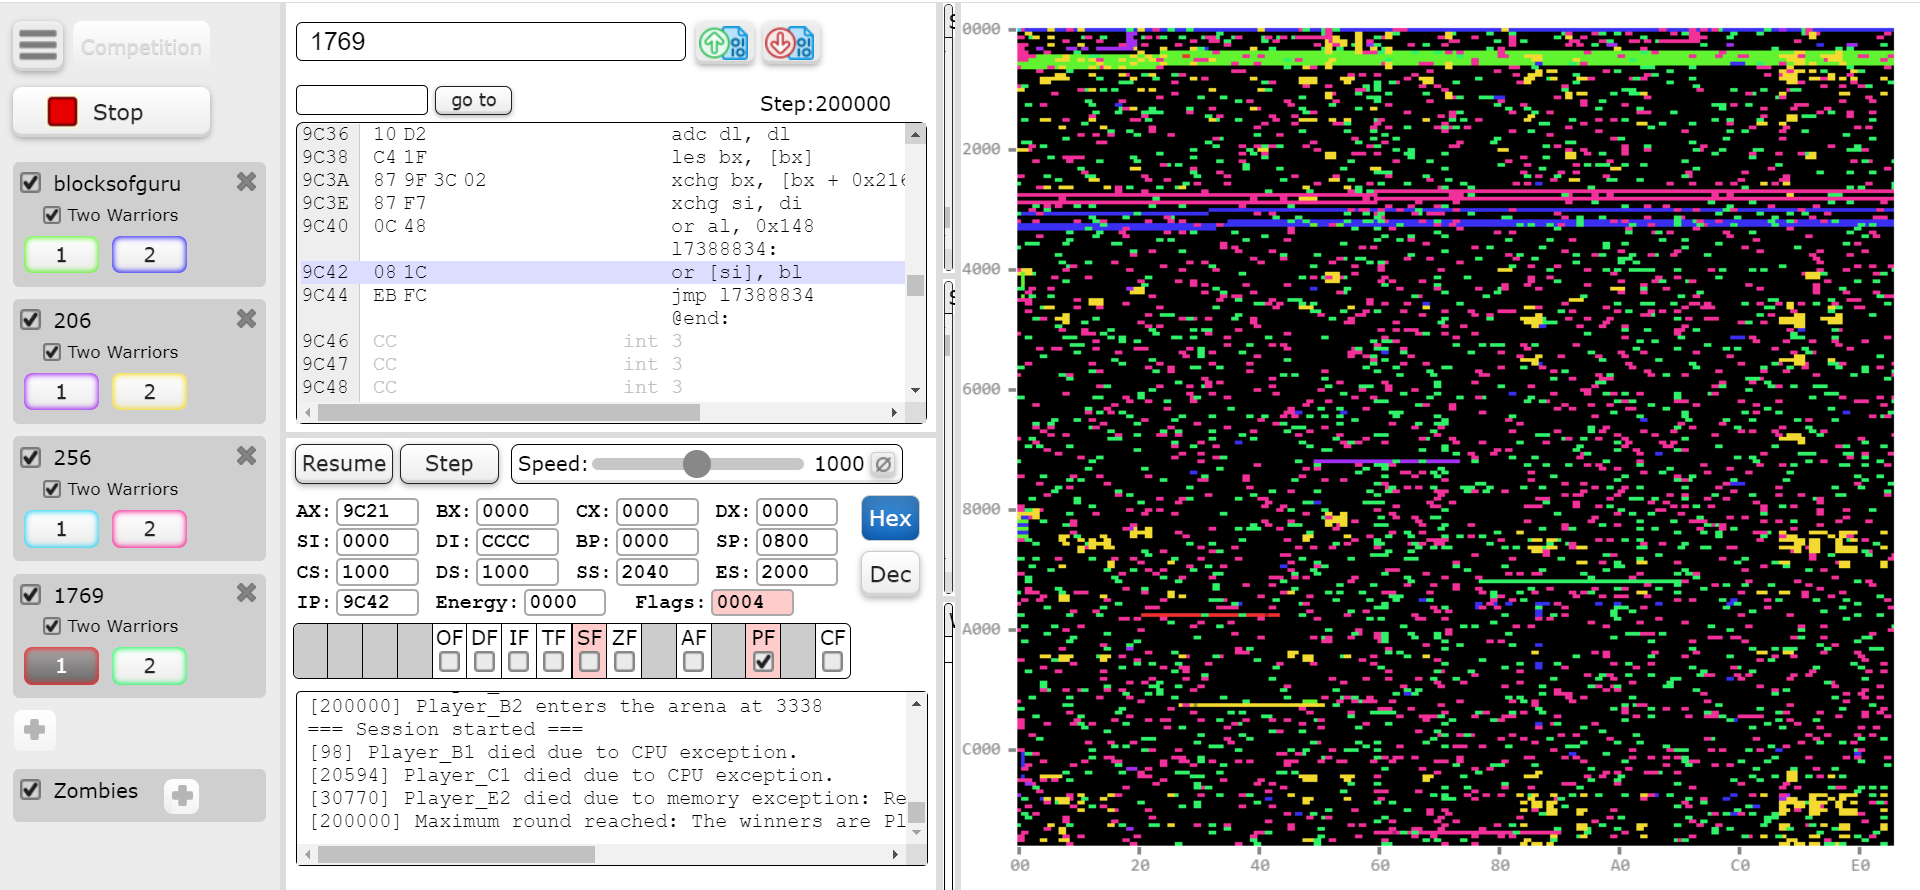
\includegraphics[width=\linewidth]{images/blocksofguru_generations_comparison_memory.png}
    \caption{Joined game memory image}
    \label{fig:joined_mem}
  \end{subfigure}
  \caption{BlocksOfGuru vs. Generation 206 vs. Generation 256 vs. Generation 1,769}
  \label{fig:joinedgame}
\end{figure}

As expected, all the evolved survivors overtook the human-written BlocksOfGuru adversary and their achieved places in \autoref{fig:joined_res} match the ones in the evolution. In \autoref{fig:joined_mem} we can see that most of memory writes were made by 1,769 and 256 best's second parts which cover the arena in green and pink. Nonetheless, 206 best's second part performed significant number of writes in yellow. All of the first part performed little to none new memory writes, as reflected in \autoref{fig:joined_mem} with neither of their colors in the arena except of the code's place.
If we take a closer look at the code, the first parts of B and C run in the loop written in their bottom, which keeps the individual alive but does not perform attacking actions -- as seen in the lack of their color in the arena. In A, both fragments run in a loop due to "jmp ax" at the end, which jumps into the beginning of the code. 
 We can see in \autoref{fig:joined_mem}, the writes A performed are concentrated in yellow areas together while the writes of B and C are scattered all across the memory image. In all of the fragments, most memory writes are performed using addressing si, yet with adding different constants. B and C use special constants like 65,535 and @start while A does not. They exceed bounds of word data and the computation is one mod $2^{16}$, which leads B and C to perform more scattered writes. Scattered writing has more chances than concentrated one to come across adversary's code, which is reflected in the higher scores B and C achieved. The evolutionary process, using its operators, was able to discover this technique and improve its off-springs along the generations.

\subsection{Vertical vs. Horizontal memory writes}
Additional fact to notice is a pattern which repeated itself in the evolved survivors. Several of them were using vertical write into memory (stride of 256 looks vertical in the engine's visualization), while the human-written ones mostly use horizontal writing patterns (consecutive bytes). As a result, the evolved survivor was able to "cut" the adversary by writing on its code before the adversary reached its code. For example, let us observe the evolved winners against Zeus and against IamAramAcham, 2006 and 2014 respectively human winners. As seen in \autoref{fig:vertical}, the evolved survivors are colored in purple and yellow and the adversary in red and green. Captures \autoref{fig:mem_before1} and \autoref{fig:mem_before2} show the initial memory image, we can only see the place the survivors code was loaded into. In captures \autoref{fig:mem_after1} and \autoref{fig:mem_after2} we can see the memory writes that were made during the battles. In both cases, the yellow and purple vertical columns "cut" the opponent's code before its red and green horizontal rows were able to reach our code. Writing vertically assures reaching the opponents code faster due to the fact most of the submitted survivors take advantage of the maximum allowed code size, thus filling at least one memory row entirely. Therefore, filling one or a few columns will be sufficient to reach the adversary's code, while writing vertically and filling row by row will take longer to find the opponent's code. Similar pattern was found also against GreeniEs 2020, Nuki’sDemons 2019, Barvaz'sAngels 2018, Memz 2017, SilentError 2015, APOCALYPSE 2008 and HutsHuts 2007.
\begin{figure}
  \centering
  \begin{subfigure}{0.48\textwidth}
    \includegraphics[width=\linewidth]{images/zeus_before_mem.png}
    \caption{Memory image before the game - Zeus}
    \label{fig:mem_before1}
  \end{subfigure}
  \hfill
  \begin{subfigure}{0.48\textwidth}
    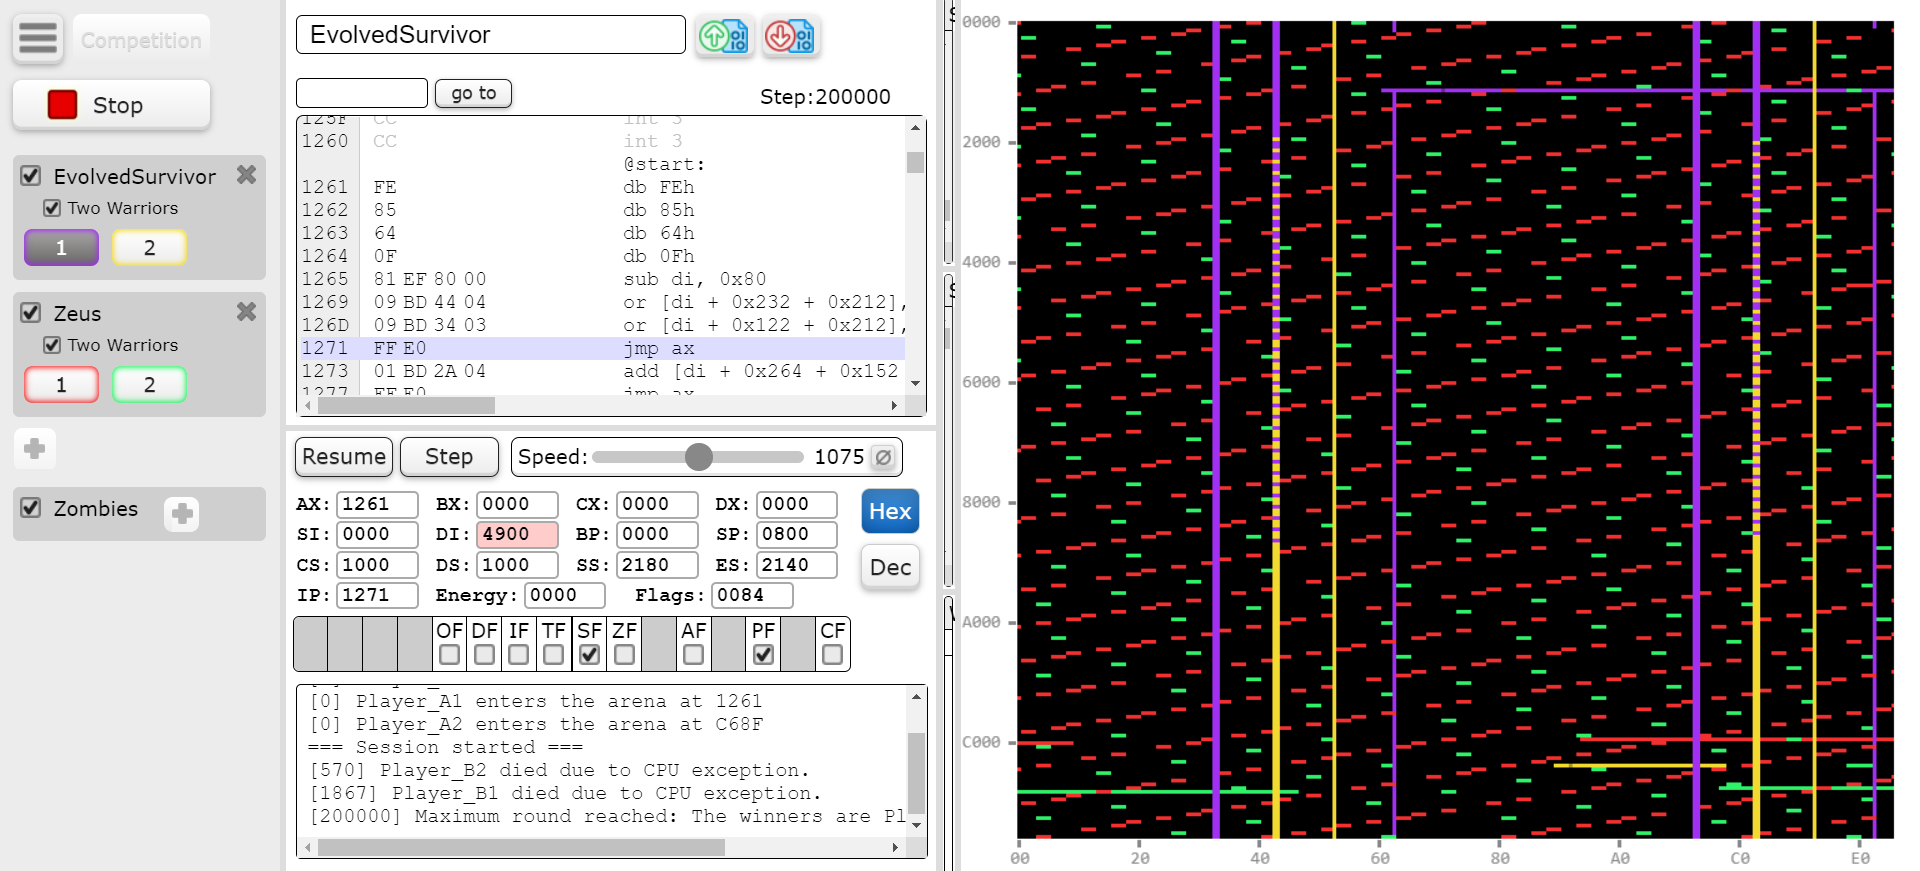
\includegraphics[width=\linewidth]{images/zeus_after_mem.png}
    \caption{Memory image after the game - Zeus}
    \label{fig:mem_after1}
  \end{subfigure}
    \begin{subfigure}{0.48\textwidth}
    \includegraphics[width=\linewidth]{images/iamaramacham_before_mem.png}
    \caption{Memory image before the game - IamAramAcham}
    \label{fig:mem_before2}
  \end{subfigure}
  \hfill
  \begin{subfigure}{0.48\textwidth}
    \includegraphics[width=\linewidth]{images/iamaramacham_after_mem.png}
    \caption{Memory image after the game - IamAramAcham}
    \label{fig:mem_after2}
  \end{subfigure}
  \caption{Vertical vs. horizontal memory write}
  \label{fig:vertical}
\end{figure}


 \subsection{Random generator pattern}
 The original program had difficulties to overtake few previous years winners -- FSM 2009, LoudBugFix 2016 and TheHeapMen 2022. Our assumption was regarding the randomness human-written survivors may use to be unpredictable and our original code did not have any element of randomness. We decided to add Pseudo-Random Number Generator (PRNG) patterns to our BNF.
 We added Linear Congruentional Generator (LCG) and XOR-Shift Generators implementation to our grammar as shown in \autoref{table3_random_set} and ran the evolution against the above adversaries again.

 \begin{table}[!ht]
\centering
\begin{tabular}{p{15.6cm}} 
<section> ::= mov ax, timestamp\\
\quad\quad\quad\quad mov <reg>, 1664525\\
\quad\quad\quad\quad mul <reg>\\
\quad\quad\quad\quad add ax, 1013904223 <section>
\\
<section> ::= mov <reg>, randint(0, 65,535)\\
\quad\quad\quad\quad mov <reg>, randint(0, 65,535)\\
\quad\quad\quad\quad xor <reg>, <reg>\\
\quad\quad\quad\quad shl <reg>, 7\\
\quad\quad\quad\quad shr <reg>, 5\\
\quad\quad\quad\quad xor <reg>, <reg> <section>
\\
\end{tabular}
\caption{Random patterns - Functions definitions}
\label{table3_random_set}
\end{table}

The randomness helped to improve overtaking only one of the three human-written survivors, LoudBugFix \autoref{table:test_random_results}. The evolved winner had the random patterns as part from its unreachable code, which means that it evolutionary helped to add it, and then 
a misfortune mutation deactivated it. We believe it helped the evolution process, even though the winning survivor doesn't actively use it. The result increased from 0.525 to 0.6475.

\begin{table}[!ht]
\centering
\begin{tabular}{|c|c|c|} 
\hline
\multicolumn{1}{|c|}{\textbf{Human-written adversary}} &
\multicolumn{1}{c|}{\textbf{Test score}} &
\multicolumn{1}{c|}{\textbf{Web score}} \\ [0.5ex] \hline\hline
LoudBugFix 2016 & 0.6475 & 541 \\ \hline
\end{tabular}
\caption{Test and web game results with random}
\label{table:test_random_results}
\end{table}

\subsection{Problematic survivors}
The most difficult survivor to overtake appeared to be FSM 2010. This survivor fills the memory from its top and bottom using horizontal lines. The uniqueness of this survivor is it almost exclusively uses the command \texttt{REP MOVSW} to write to the memory, The ability of the evolved survivor to hit exactly this line in its code is low, thus we were able to reach a tie but not a win.

\subsection{Purely random code evolution}
We compared our G3P with a restricted version of the grammar. We only provided the possibility to evolve commands consisting of dw declarations, which results in purely random assembly code generation. As each assembly command has its representation in hex value, the evolved programs will be legal. The goal was to find out if the provided language structures and patterns were helpful to the evolution or perhaps it could have learned them during the process. Except of this change, all of the evolutionary process was left the same. The chosen adversary was a defensive survivor consisting of an empty infinite loop. In order to overtake it, a survivor must perform memory writes. After a full run of 2,000 generation, the dw evolution was able to achieve a tie -- it managed to learn an original way to create a loop as seen in the resulted code and its translation in \autoref{random_evolution}. Note that the \texttt{JMP [BP+SI]} acts as \texttt{JMP [AX]} which makes it infinite loop. This is an impressive result, however our original process managed to win this opponent immediately. Perhaps with more time and resources, success of dw evolution might be achieved.

\begin{figure}
\centering
\begin{subfigure}[t]{0.48\textwidth}
    \begin{assembly}
    @start:
    dw 0x94
    dw 0x258
    dw 0x224
    dw 0x182
    dw 0x144
    dw 0x222
    dw 0x54
    dw 0x132
    dw 0x198
    dw 0x190
    dw 0x134
    dw 0x104
    dw 0x256
    dw 0x134
    dw 0x70
    dw 0x244
    dw 0x178
    dw 0x144
    ...
    \end{assembly}
    \caption{Evolved dw code}
\end{subfigure}
\hfill
\begin{subfigure}[t]{0.49\textwidth}
    \begin{assembly}
    @start:
    XCHG SP, AX
    ADD [BX + SI + 0x2], BL
    AND AL, 0x2
    ADD BYTE [BX + DI], 0x44
    ADD [BP + SI], SP
    ADD DL, [SI + 0x0]
    XOR AL,[BX + DI]
    CBW
    ADD [BX + SI + 0x3401], DX
    ADD [SI], AX
    ADD [BP + 0x2], DX
    XOR AL, 0x1
    JO SHORT 0x2
    INC SP
    ADD BH, [BX + SI + 0x1]
    INC SP
    ADD SP, BP
    JMP [BP + SI]
    ...
    \end{assembly}
    \caption{Translation to Assembly}
\end{subfigure}
\caption{Purely random assembly code generation result}
\label{random_evolution}
\end{figure}

\subsection{Comparison to ChatGPT}
Another comparison was made to ChatGPT's, one of toady's leading LLMs. Using prompt engineering, we explained CodeGuru game, the special opcodes and the rules and asked for a survivor with best chance to overtake others. The evolution of the suggested survivors was performed against the example survivors of the competition in the web engine of the game. First provided survivors didn't compile, after supplying corrections they compiled however achieved poor scores. Even when the opponents code was supplied to ChatGPT, its produced survivor didn't manage to win.

These results show a primary success in automatic evolution of assembly code in adversarial environment. The results demonstrate G3P power to find a weakness in adversary code and utilize it to a defined goal. In our case, it was to win a CodeGuru game, however, any other goal can be defined through modifying the fitness calculation and minor grammar modifications.


\section{Discussion}
Our results open the road for various goals to be achieved automatically by code generation using GP. We believe this work has a significant impact on the Cyber-Security world. As assembly is a language widely used, by just adjusting the fitness evaluation, the evolved code can be intended to avoid security mechanisms or on the contrary find suspicious adversary code. It can be applied in wide range of domains. Furthermore, any language that can be represented similarly to assembly using BNF can be used for the evolution. The uniqueness of our work is expressed in the minimal assumptions which are required for the process -- a definition of language BNF and a goal for evaluating individuals by it, are sufficient for evolving a program which fulfills the desired goal. 

\bibliographystyle{ACM-Reference-Format}
\bibliography{references}  
\end{document}
